\documentclass[a4paper,twoside]{article}
\usepackage{blindtext}  
\usepackage{geometry}

% Chinese support
\usepackage[UTF8, scheme = plain]{ctex}

% Page margin layout
\geometry{left=2.3cm,right=2cm,top=2.5cm,bottom=2.0cm}


\usepackage{listings}
\usepackage{xcolor}
\usepackage{geometry}
\usepackage{amsmath}
\usepackage{float}
\usepackage{hyperref}

\usepackage{graphics}
\usepackage{graphicx}
\usepackage{subfigure}
\usepackage{epsfig}
\usepackage{float}

\usepackage{algorithm}
\usepackage[noend]{algpseudocode}

\usepackage{booktabs}
\usepackage{threeparttable}
\usepackage{longtable}
\usepackage{listings}
\usepackage{tikz}

% cite package, to clean up citations in the main text. Do not remove.
\usepackage{cite}

\usepackage{color,xcolor}

%% The amssymb package provides various useful mathematical symbols
\usepackage{amssymb}
%% The amsthm package provides extended theorem environments
\usepackage{amsthm}
\usepackage{amsfonts}
\usepackage{enumerate}
\usepackage{enumitem}
\usepackage{listings}

\usepackage{indentfirst}
\setlength{\parindent}{2em} % Make two letter space in the first paragraph
\usepackage{setspace}
\linespread{1.5} % Line spacing setting
\usepackage{siunitx}
\setlength{\parskip}{0.5em} % Paragraph spacing setting

% \usepackage[contents =22920202204622, scale = 10, color = black, angle = 50, opacity = .10]{background}

\renewcommand{\figurename}{图}
\renewcommand{\lstlistingname}{代码} 
\renewcommand{\tablename}{表格}
\renewcommand{\contentsname}{目录}
\floatname{algorithm}{算法}

\graphicspath{ {images/} }

%%%%%%%%%%%%%
\newcommand{\StudentNumber}{22920202204622}  % Fill your student number here
\newcommand{\StudentName}{熊恪峥}  % Replace your name here
\newcommand{\PaperTitle}{作业(七)}  % Change your paper title here
\newcommand{\PaperType}{算法设计与分析} % Replace the type of your report here
\newcommand{\Date}{2022年4月13日}
\newcommand{\College}{信息学院}
\newcommand{\CourseName}{算法设计与分析}
%%%%%%%%%%%%%

%% Page header and footer setting
\usepackage{fancyhdr}
\usepackage{lastpage}
\pagestyle{fancy}
\fancyhf{}
% This requires the document to be twoside
\fancyhead[LO]{\texttt{\StudentName }}
\fancyhead[LE]{\texttt{\StudentNumber}}
\fancyhead[C]{\texttt{\PaperTitle }}
\fancyhead[R]{\texttt{第{\thepage}页,共\pageref*{LastPage}页}}


\title{\PaperTitle}
\author{\StudentName}
\date{\Date}

\lstset{
	basicstyle          =   \sffamily,          % 基本代码风格
	keywordstyle        =   \bfseries,          % 关键字风格
	commentstyle        =   \rmfamily\itshape,  % 注释的风格,斜体
	stringstyle         =   \ttfamily,  % 字符串风格
	flexiblecolumns,                % 别问为什么,加上这个
	numbers             =   left,   % 行号的位置在左边
	showspaces          =   false,  % 是否显示空格,显示了有点乱,所以不现实了
	numberstyle         =   \zihao{-5}\ttfamily,    % 行号的样式,小五号,tt等宽字体
	showstringspaces    =   false,
	captionpos          =   t,      % 这段代码的名字所呈现的位置,t指的是top上面
	frame               =   lrtb,   % 显示边框
}

\lstdefinestyle{PythonStyle}{
	language        =   Python, % 语言选Python
	basicstyle      =   \zihao{-5}\ttfamily,
	numberstyle     =   \zihao{-5}\ttfamily,
	keywordstyle    =   \color{blue},
	keywordstyle    =   [2] \color{teal},
	stringstyle     =   \color{magenta},
	commentstyle    =   \color{red}\ttfamily,
	breaklines      =   true,   % 自动换行,建议不要写太长的行
	columns         =   fixed,  % 如果不加这一句,字间距就不固定,很丑,必须加
	basewidth       =   0.5em,
}

\algnewcommand\algorithmicinput{\textbf{Input:}}
\algnewcommand\algorithmicoutput{\textbf{Output:}}
\algnewcommand\Input{\item[\algorithmicinput]}%
\algnewcommand\Output{\item[\algorithmicoutput]}%

\usetikzlibrary{positioning, shapes.geometric}

\begin{document}
	
%%%%%%%%%%%%%%%%%%%%%%%%%%%%%%%%%%%%%%%%%%%%
\makeatletter % change default title style
\renewcommand*\maketitle{%
	\begin{center} 
		\bfseries  % title 
		{\LARGE \@title \par}  % LARGE typesetting
		\vskip 1em  %  margin 1em
		{\global\let\author\@empty}  % no author information
		{\global\let\date\@empty}  % no date
		\thispagestyle{empty}   %  empty page style
	\end{center}%
	\setcounter{footnote}{0}%
}
\makeatother
%%%%%%%%%%%%%%%%%%%%%%%%%%%%%%%%%%%%%%%%%%%%
	
	
\thispagestyle{empty}

\vspace*{1cm}

\begin{figure}[h]
	\centering
	
\includegraphics[width=4.0cm]{logo.png}
\end{figure}

\vspace*{1cm}

\begin{center}
	\Huge{\textbf{\PaperType}}
	
	\Large{\PaperTitle}
\end{center}

\vspace*{1cm}

\begin{table}[h]
	\centering	
	\begin{Large}
		\renewcommand{\arraystretch}{1.5}
		\begin{tabular}{p{3cm} p{5cm}<{\centering}}
			姓\qquad 名 & \StudentName  \\
			\hline
			学\qquad号 & \StudentNumber \\
			\hline
			日\qquad期 & \Date  \\
			\hline
			学\qquad院 & \College  \\
			\hline
			课程名称 & \CourseName  \\
			\hline
		\end{tabular}
	\end{Large}
\end{table}

\newpage

\title{
	\Large{\textcolor{black}{\PaperTitle}}
}
	
	
\maketitle
	
\tableofcontents
 
\newpage
\setcounter{page}{1}

\begin{spacing}{1.2}

\section{题8.3}

使用邻接矩阵存图,图的转置就是矩阵的转置,因此可以直接使用矩阵的转置来求解。
这种方法的时间复杂度是$\mathcal{O}(\|V\|^2)$,如算法~\ref{algo:transpose_mat}。

\begin{algorithm}
	\caption{转置邻接矩阵}
	\label{algo:transpose_mat}
	\begin{algorithmic}[1]
		\Input{邻接矩阵$M$}
		
		\Procedure{Transpose}{$M$}     

		\State $V \gets \Call{Vertices}{$M$}$
		\State $T \gets \Call{EmptyMatrix}{$V$}$


		\For{$i = 1 \to |V|$}
			\For{$j = 1 \to |V|$}
				\State $T[i,j] \gets M[j,i]$
			\EndFor
		\EndFor

		\State \Return $T$
		
		\EndProcedure
	\end{algorithmic}
\end{algorithm}	

使用邻接表存图,可以通过遍历每个顶点的邻接表并将反向边插入新图中实现,
这种方法的时间复杂度是$\mathcal{O}(\|V\|+\|E\|)$,如算法~\ref{algo:transpose_adjlist}。

\begin{algorithm}
	\caption{转置邻接表}
	\label{algo:transpose_adjlist}
	\begin{algorithmic}[1]
		\Input{邻接表$G$}
		
		\Procedure{Transpose}{$G$}     
		\State $GT.Vertices\gets G.Vertices$

		\For{$v \in G.Vertices$}
			\State $GT.Adj[v] \gets$ \Call{EmptyList}{}
			\For{$e \in G.Adj[v]$}
				\State $GT.Adj[e.V2] \gets (e.V2,e.V1)$
			\EndFor
		\EndFor
		\EndProcedure
	\end{algorithmic}
\end{algorithm}	

\section{题8.4}

如图~\ref{fig:t84_example},以$a$为源点进行深度优先遍历,得到的$d(u)$如表~\ref{tbl:du}

\begin{figure}[htbp]
	\centering
	\label{fig:t84_example}
	\subfigure[无向图$G$]{
		\centering
		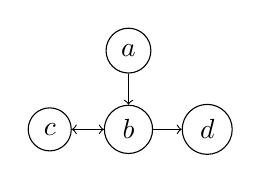
\begin{tikzpicture}[main/.style = {draw, circle}] 
			\node[main] (a) {$a$}; 
			\node[main] (b) [below of=a] {$b$}; 
			\node[main] (c) [left of=b] {$c$}; 
			\node[main] (d) [right of=b] {$d$}; 
			\draw[->] (a) -- (b);
			\draw[->] (c) -- (b);
			\draw[->] (b) -- (d);
			\draw[->] (b) -- (c);
		\end{tikzpicture} 
	}
	~
	\subfigure[产生的搜索树]{
		\centering
		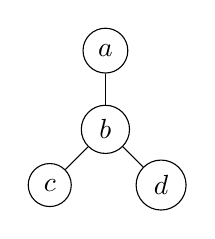
\begin{tikzpicture}[main/.style = {draw, circle}] 
			\node[main] (a) {$a$}; 
			\node[main] (b) [below of=a] {$b$}; 
			\node[main] (c) [below left of=b] {$c$}; 
			\node[main] (d) [below right of=b] {$d$}; 
			\draw (a) -- (b);
			\draw (b) -- (c);
			\draw (b) -- (d);
		\end{tikzpicture} 
	}
	\caption{反例}
\end{figure}

\begin{table}[H]
	\centering
	\label{tbl:du}
	\begin{tabular}{ccccc}
		\toprule
		$u$ & $a$ & $b$ & $c$ & $d$ \\
		\midrule
		$d(u)$ & $1$ & $2$ & $3$ & $4$ \\
		\bottomrule
	\end{tabular}
	\caption{深度优先遍历得到的$d(u)$}
\end{table}

可见$d(c)>d(d)$,且$c$到$d$存在路径,但$d$不是$c$的子顶点。

\section{题8.6}

Tarjan算法可以在$\mathcal{O}(\|V\|+\|E\|)$的时间里求出强连通分量。对无向图中的每一个
顶点使用算法~\ref{algo:tarjan},可以求出强连通分量。

\begin{algorithm}
	\caption{Tarjans算法}
	\label{algo:tarjan}
	\begin{algorithmic}[1]		
		\Procedure{Tarjan}{$G$}     
		\State $GT.Vertices\gets G.Vertices$

		\EndProcedure
	\end{algorithmic}
\end{algorithm}	

\section{题8.7}

Floyd算法的修改版可以用来计算传递闭包,如算法\ref{algo:floyd_closure}。

\begin{algorithm}
	\caption{Floyd算法求传递闭包}
	\label{algo:floyd_closure}
	\begin{algorithmic}[1]		
		\Procedure{Floyd}{$G$}     
		\State $GT.Vertices\gets G.Vertices$

		\EndProcedure
	\end{algorithmic}
\end{algorithm}

\section{题8.11}

存在一些图使得$Prim$算法慢于$Kruskal$算法。当使用的排序算法足够好时,$Kruskal$算法
的时间复杂度时$\mathcal{O}(\|E\|\log \|E\|)$,而$Prim$算法的时间复杂度是$\mathcal{O}(\|V\|^2)$。
因此,对于顶点多而边少的图,$Prim$算法比$Kruskal$算法慢。

\section{题8.12}

当图中存在负环时$i$到$j$无最短路径。如图~\ref{fig:negcircle}。

\begin{figure}[htbp]
	\centering
	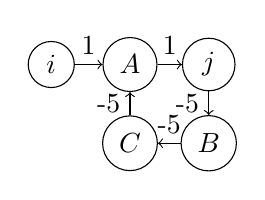
\begin{tikzpicture}[main/.style = {draw, circle}] 
		\node[main] (i) {$i$}; 
		\node[main] (1) [right of=i] {$A$}; 
		\node[main] (j) [right of=1] {$j$}; 
		\node[main] (2) [below of=j] {$B$}; 
		\node[main] (3) [left of=2] {$C$}; 

		\draw[->] (i) edge node[above,draw=none,fill=none]{1} (1);
		\draw[->] (1) edge node[above,draw=none,fill=none]{1} (j);
		\draw[->] (j) edge node[left,draw=none,fill=none]{-5} (2);
		\draw[->] (2) edge node[above,draw=none,fill=none]{-5} (3);
		\draw[->] (3) edge node[left,draw=none,fill=none]{-5} (1);
	
	\end{tikzpicture} 
	\caption{反例}
	\label{fig:negcircle}
\end{figure}

\section{题8.13}

实现该功能,只需要遍历所有的边,并比较是否有不满足三角形不等式的距离,即
$d[v]>d[u]+w(u,v)$。如算法\ref{algo:bellmanford}。

\begin{algorithm}[H]
	\caption{Bellmanford算法}
	\label{algo:bellmanford}
	\begin{algorithmic}[1]		
		\Procedure{Bellmanford}{$G,w,s$}     
		\For{$i\gets 1 \to \|V\|-1$}
			\For{$each \ edge(u,v)\in E$}
			\State \Call{Relax}{u,v,w}
			\EndFor
		\EndFor
		\For{$each \ edge(u,v)\in E$}
			\If{$d[v]>d[u]+w(u,v)$}
				\State $d[v]\gets \infty$
				\State \Return $0$
			\EndIf
		\EndFor
		\State \Return $1$
		\EndProcedure
	\end{algorithmic}
\end{algorithm}	

\section{题8.14}

为了求出DAG中的路径数量,首先进行拓扑排序然后按由逆拓扑序递推可以求出任意两点$s, t$间的路径数量。

\begin{equation}
	f[i]=
	\begin{cases}
		1 \ \ i=t \\
		f[i]+\sum_{(i,v)\in E} f[v] \ \ i\neq t
	\end{cases}
\end{equation}

然后对起点$s$和任意点求路径数并求和,就可以得到路径树,如算法~\ref{algo:countofpath}。

\begin{algorithm}
	\caption{计算路径数}
	\label{algo:countofpath}
	\begin{algorithmic}[1]		
		\Procedure{PathCount}{$G,s$}     
		\State $GT.Vertices\gets G.Vertices$

		\EndProcedure
	\end{algorithmic}
\end{algorithm}	

\section{题8.16}

当第一次$Relax$操作未能改变$d[v]$时停止,则可以得到最小边数的最大值。如算法~\ref{algo:maxedgecount}

\begin{algorithm}
	\caption{计算最小边数最大值}
	\label{algo:maxedgecount}
	\begin{algorithmic}[1]		
		\Procedure{Bellmanford}{$G,s$}     
		\State $GT.Vertices\gets G.Vertices$

		\EndProcedure
	\end{algorithmic}
\end{algorithm}

\section{题8.20}

算法仍然正确。

\begin{proof}

	设最后一个顶点为$u$,如果$u$到$s$不可达,则$d[u]\gets \infty=\delta(s,u)$

	如果$u$到$s$可达,则存在路径$p$,从$s$经过点$m$到达$u$,由于$d[x]=\delta(s,x)$,
	则按路径松弛性质,$d[u]=\delta(s,u)$

	则算法正确
\end{proof}

\section{题8.24}

为了构造最优解,需要在每次成功松弛的时候记录松弛的点。如算法~\ref{algo:floyd2}

\begin{algorithm}
	\caption{计算最小边数最大值}
	\label{algo:floyd2}
	\begin{algorithmic}[1]		
		\Procedure{Floyd}{$G$}     
		\State $GT.Vertices\gets G.Vertices$

		\EndProcedure
	\end{algorithmic}
\end{algorithm}


\section{题8.25}
每次迭代生成的矩阵如表:

\section{题8.26}

该算法需要存储$d_{ij}$,由于$i\le\|V\|,j\le\|V\|$,则所需空间为$\mathcal{O}(\|V\|^2)$。

该算法的正确性证明如下

\begin{proof}
	
\end{proof}

\section{题8.27}

由松弛方法可知,可以调用两次Floyd算法,如果调用完第二次,有路径长度被再一次更新,则说明存在负环。

\end{spacing}

\end{document}